In order to perform probabilistic or scenario risk calculations, it is
necessary to define a \gls{vulnerabilityfunction} for each building typology
present in the \gls{exposuremodel}. In this section, the schema for the
\gls{vulnerabilitymodel} is described in detail. A graphical representation of
a \gls{vulnerabilitymodel} (mean loss ratio for a set of intensity measure
levels) is illustrated in Figure~\ref{fig:vulnerability-zero-cov}.

\begin{figure}[ht]
\centering
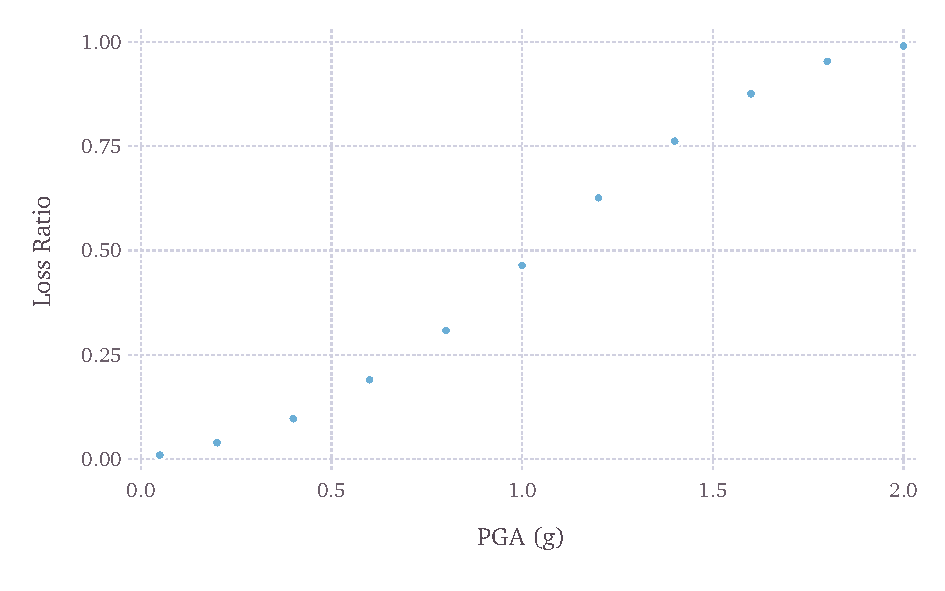
\includegraphics[width=12cm]{figures/risk/vulnerability-zero-cov.pdf}
\caption{Graphical representation of a vulnerability model}
\label{fig:vulnerability-zero-cov}
\end{figure}


Note that although the uncertainty for each loss ratio is not represented in
Figure~\ref{fig:vulnerability-zero-cov}, it can be considered in the input
file, by means of a coefficient of variation per loss ratio and a
probabilistic distribution, which can currently be set to lognormal~(LN),
Beta~(BT); or by specifying a discrete probability mass~(PM)\footnote{As of
\glsdesc{acr:oqe18}, the ``PM'' option for defining
\glspl{vulnerabilityfunction} is supported by the Scenario Risk and the
Stochastic Event-Based Probabilistic Risk Calculators, but not by the
Classical Probabilistic Risk Calculator.} distribution of the loss ratio at a
set of intensity levels. An example of a \gls{vulnerabilityfunction} that
models the uncertainty in the loss ratio at different intensity levels using a
lognormal distribution is illustrated in 
Figure~\ref{fig:vulnerability-nonzero-cov}.

\begin{figure}[ht]
\centering
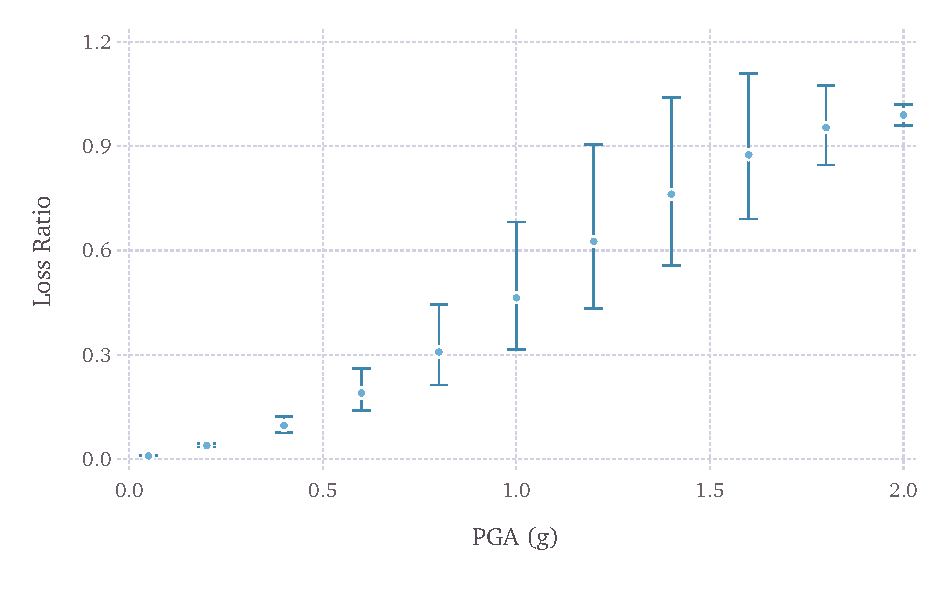
\includegraphics[width=12cm]{figures/risk/vulnerability-nonzero-cov.pdf}
\caption{Graphical representation of a vulnerability function that models the uncertainty in the loss ratio using a lognormal distribution. The mean loss ratios and coefficients of variation are illustrated for a set of intensity levels.}
\label{fig:vulnerability-nonzero-cov}
\end{figure}

In general, defining \glspl{vulnerabilityfunction} requires the user to
specify the distribution of the loss ratio for a set of intensity levels. The
loss ratio distributions can be defined using either a discrete or a
continuous format, and the \gls{vulnerabilitymodel} file can include a mix of
both types of \glspl{vulnerabilityfunction}. It is also possible to define a
\gls{vulnerabilityfunction} using a set of deterministic loss ratios
corresponding to a set of intensity levels (i.e., ignoring the uncertainty in
the conditional loss ratios).

An example \gls{vulnerabilitymodel} comprising three
\glspl{vulnerabilityfunction} is shown in
Listing~\ref{lst:input_vulnerability}. This \gls{vulnerabilitymodel} contains
one function that uses the lognormal distribution to represent the uncertainty
in the loss ratio at different intensity levels, one function that uses the
Beta distribution, and one function that is defined using a discrete
probability mass distribution.

\begin{listing}[htbp]
  \inputminted[firstline=1,firstnumber=1,fontsize=\footnotesize,frame=single,linenos,bgcolor=lightgray]{xml}{oqum/risk/verbatim/input_vulnerability.xml}
  \caption{Example vulnerability model (\href{https://raw.githubusercontent.com/GEMScienceTools/oq-engine-docs/master/oqum/risk/verbatim/input_vulnerability.xml}{Download example})}
  \label{lst:input_vulnerability}
\end{listing}


The initial portion of the schema contains general information that describes
some general aspects of the \gls{vulnerabilitymodel}. The information in this
metadata section is common to all of the functions in the
\gls{vulnerabilitymodel} and needs to be included at the beginning of every
\gls{vulnerabilitymodel} file. The parameters are illustrated in the snippet
shown and described below:

\inputminted[firstline=4,firstnumber=4,lastline=8,fontsize=\footnotesize,frame=single,linenos,bgcolor=lightgray]{xml}{oqum/risk/verbatim/input_vulnerability.xml}

\begin{itemize}

  \item \Verb+id+: a unique string (ASCII) used to identify the
    \gls{vulnerabilitymodel}. This string can contain letters~(a--z; A--Z),
    numbers~(0--9), dashes~(-), and underscores~(\_), with a maximum of
    100~characters.

  \item \Verb+assetCategory+: an optional string (ASCII) used to specify the
    type of \glspl{asset} for which \glspl{vulnerabilityfunction} will be 
    defined in this file (e.g: buildings, lifelines).

  \item \Verb+lossCategory+: mandatory; valid strings for this attribute are 
    ``structural'', ``nonstructural'', ``contents'',  
    ``business\_interruption'', and ``occupants''.

  \item \Verb+description+: mandatory; a brief string with further information about the
    \gls{vulnerabilitymodel}, for example, which building typologies are 
    covered or the source of the functions in the \gls{vulnerabilitymodel}.

\end{itemize}


The following snippet from the above \gls{vulnerabilitymodel} example file defines
a \gls{vulnerabilityfunction} modelling the uncertainty in the conditional loss
ratios using a (continuous) lognormal distribution:

\inputminted[firstline=10,firstnumber=10,lastline=14,fontsize=\footnotesize,frame=single,linenos,bgcolor=lightgray]{xml}{oqum/risk/verbatim/input_vulnerability.xml}

The following attributes are needed to define a \gls{vulnerabilityfunction} which
uses a continuous distribution to model the uncertainty in the conditional
loss ratios:

\begin{itemize}

  \item \Verb+id+: a unique string (ASCII) used to identify the \gls{taxonomy} for 
    which the function is being defined. This string is used to relate the 
    \gls{vulnerabilityfunction} with the relevant \gls{asset} in the 
    \gls{exposuremodel}. This string can contain letters~(a--z; A--Z), 
    numbers~(0--9), dashes~(-), and underscores~(\_), with a maximum of
    100~characters.

  \item \Verb+dist+: mandatory; for \glspl{vulnerabilityfunction} which use a continuous 
    distribution to model the uncertainty in the conditional loss ratios, 
    this attribute should be set to either ``\Verb+LN+'' if using the lognormal
    distribution, or to ``\Verb+BT+'' if using the Beta distribution.

  \item \Verb+imls+: mandatory; this attribute specifies the list of intensity levels
    for which the parameters of the conditional loss ratio distributions will
    be defined. In addition, it is also necessary to define the intensity 
    measure type (\Verb+imt+).

  \item \Verb+meanLRs+: mandatory; this field is used to define the mean loss ratios
    for this \gls{vulnerabilityfunction} for each of the intensity levels
    defined by the attribute \Verb+imls+. The number of mean loss ratios
    defined by the \Verb+meanLRs+ attribute must be equal to the number of
    intensity levels defined by the attribute \Verb+imls+.

  \item \Verb+covLRs+: mandatory; this field is used to define the coefficient of 
    variation for the conditional distribution of the loss ratios for this
    \gls{vulnerabilityfunction} for each of the intensity levels defined by
    the attribute \Verb+imls+. The number of coefficients of variation of loss
    ratios defined by the \Verb+covLRs+ attribute must be equal to the number
    of intensity levels defined by the attribute \Verb+imls+. The uncertainty
    in the conditional loss ratios can be ignored by setting all of the
    \Verb+covLRs+ for a given \gls{vulnerabilityfunction} to zero.

\end{itemize}


The next snippet from the \gls{vulnerabilitymodel} example file of
Listing~\ref{lst:input_vulnerability} defines a \gls{vulnerabilityfunction}
which models the uncertainty in the conditional loss ratios using a
(discrete) probability mass distribution:

\inputminted[firstline=24,firstnumber=24,lastline=33,fontsize=\footnotesize,frame=single,linenos,bgcolor=lightgray]{xml}{oqum/risk/verbatim/input_vulnerability.xml}

The following attributes are needed to define a \gls{vulnerabilityfunction}
which uses a discrete probability mass distribution to model the uncertainty
in the conditional loss ratios:

\begin{itemize}

  \item \Verb+id+: a unique string (ASCII) used to identify the \gls{taxonomy} for 
    which the function is being defined. This string is used to relate the 
    \gls{vulnerabilityfunction} with the relevant \gls{asset} in the 
    \gls{exposuremodel}. This string can contain letters~(a--z; A--Z), 
    numbers~(0--9), dashes~(-), and underscores~(\_), with a maximum of
    100~characters.

  \item \Verb+dist+: mandatory; for \glspl{vulnerabilityfunction} which use a 
    discrete probability mass distribution to model the uncertainty in the
    conditional loss ratios, this attribute should be set to ``\Verb+PM+''.

  \item \Verb+imls+: mandatory; this attribute specifies the list of intensity levels
    for which the parameters of the conditional loss ratio distributions will
    be defined. In addition, it is also necessary to define the intensity 
    measure type (\Verb+imt+).

  \item \Verb+probabilities+: mandatory; this field is used to define the
    probability of observing a particular loss ratio (specified for each row of
    \Verb+probabilities+ using the attribute \Verb+lr+), conditional on the set
    of intensity levels specified using the attribute \Verb+imls+.
    for this \gls{vulnerabilityfunction}. Thus, the number of probabilities
    defined by each \Verb+probabilities+ attribute must be equal to the number
    of intensity levels defined by the attribute \Verb+imls+. On the other hand,
    there is no limit to the number of loss ratios for which
    \Verb+probabilities+ can be defined. In the example shown here, notice that
    the set of probabilities conditional on any particular intensity level,
    say, $MMI = 8$, sum up to one.

\end{itemize}


Note that the schema for representing \glspl{vulnerabilitymodel} has changed
between \gls{acr:nrml} v0.4 (used prior to \gls{acr:oqe17}) and \gls{acr:nrml}
v0.5 (introduced in \gls{acr:oqe17}).

A deprecation warning is printed every time you attempt to use a
\gls{vulnerabilitymodel} in the old \gls{acr:nrml} v0.4 format in an
\gls{acr:oqe17} (or later) risk calculation. To get rid of the warning you
must upgrade the old \glspl{vulnerabilitymodel} files to \gls{acr:nrml} v0.5.
You can use the command \Verb+upgrade_nrml+ with oq to do this as
follows:

\begin{minted}[fontsize=\footnotesize,frame=single,bgcolor=lightgray]{shell-session}
user@ubuntu:~\$ oq upgrade_nrml <directory-name>
\end{minted}

The above command will upgrade all of your old \gls{vulnerabilitymodel} files to
\gls{acr:nrml} v0.5. The original files will be kept, but with a .bak extension
appended. Notice that you will need to set the \Verb+lossCategory+ attribute
to its correct value manually. This is easy to do, since if you try to run a
computation you will get a clear error message telling the expected value for
the \Verb+lossCategory+ for each file.


Several methodologies to derive \glspl{vulnerabilityfunction} are currently being
evaluated by \gls{acr:gem} and have been included as part of the Risk
Modeller's Toolkit, the code for which can be found on a public repository at
GitHub at: 
\href{http://github.com/gemsciencetools/rmtk}{http://github.com/gemsciencetools/rmtk}.

A web-based tool to build an \gls{vulnerabilitymodel} in the \gls{acr:nrml} schema
are also under development, and can be found at the OpenQuake platform at the
following address: \href{https://platform.openquake.org/ipt/}{https://platform.openquake.org/ipt/}.
